\documentclass[12pt, a4paper]{article}

% ─────────────────────────────────────────────────────────────────────────────
% arXiv compatibility
% ─────────────────────────────────────────────────────────────────────────────
\usepackage[margin=1in]{geometry}
\usepackage[T1]{fontenc}
\usepackage{ae,aecompl}
\usepackage{times}
\usepackage{helvet}
\usepackage{courier}
\usepackage[utf8]{inputenc}
\usepackage{flushend}
\usepackage{natbib}
\bibliographystyle{aea}

% ─────────────────────────────────────────────────────────────────────────────
% Math & Tables
% ─────────────────────────────────────────────────────────────────────────────
\usepackage{amsmath, amssymb, amsthm}
\usepackage{booktabs}
\usepackage{threeparttable}
\usepackage{graphicx}
\usepackage{hyperref}
\usepackage{algorithm}
\usepackage{algpseudocode}
\usepackage[dvipsnames]{xcolor}
\hypersetup{
    colorlinks=true,
    linkcolor=blue,
    citecolor=blue,
    urlcolor=blue
}

% ─────────────────────────────────────────────────────────────────────────────
% Title / Authors / Abstract
% ─────────────────────────────────────────────────────────────────────────────
\title{\textbf{FinAI: An AI-Powered Research Workflow for Economic and Financial Studies}}
\author{%
    Xu Zheyi\thanks{Corresponding author. Email: \href{mailto:yi1353370501@gmail.com}{yi1353370501@gmail.com}. ORCID: \href{https://orcid.org/0009-0000-3428-816X}{0009-0000-3428-816X}.}%
    \quad
    Central South University\\
    Changsha, China
}
\date{\today}

\begin{document}

\maketitle

\begin{abstract}
We introduce \textbf{FinAI}, an end-to-end AI-powered research workflow designed for economic and financial research. FinAI integrates large language models with 43 data-source servers, modern causal inference implementations, and automated paper drafting to accelerate the research pipeline from idea generation to submission-ready manuscript. We document the system's architecture, benchmark its econometric implementations against analytical references (5/5 tests pass with MAD < 0.05), and demonstrate its capabilities through three case studies in green finance, carbon economics, and digital finance. FinAI reduces literature review time by approximately 20x, empirical design time by approximately 15x, and LaTeX formatting time by approximately 100x compared to manual workflows. All generated outputs require human review before submission. The system is open-source and available at \url{https://github.com/csmar432/finai-research}. Zenodo archive: \href{https://doi.org/10.5281/zenodo.21262689}{10.5281/zenodo.21262689}.
\end{abstract}

\textbf{Keywords:} AI for science, causal inference, difference-in-differences, research automation, large language models, econometrics

\textbf{JEL Codes:} C18, G00, O30

\newpage

% ─────────────────────────────────────────────────────────────────────────────
% 1. INTRODUCTION
% ─────────────────────────────────────────────────────────────────────────────
\section{Introduction}

Academic research in economics and finance is increasingly data-intensive, requiring integration of multiple data sources, application of sophisticated econometric methods, and adherence to rigorous formatting standards for publication. The median time from research question to first submission is 12--18 months for junior researchers, with literature review, data collection, and manuscript preparation consuming the majority of this time.

Large language models (LLMs) offer a new paradigm for accelerating research. However, general-purpose LLMs lack domain-specific knowledge for econometric method selection, real-time access to financial databases, and familiarity with journal-specific formatting requirements.

We develop \textbf{FinAI}, a purpose-built AI research assistant that addresses these gaps. FinAI combines:

\begin{enumerate}
    \item \textbf{43 MCP server directories} providing structured access to A-share financial data, US equity data, global macro indicators (FRED, World Bank, IMF, OECD), and 200M+ academic papers.
    \item \textbf{20+ econometric implementations} covering modern causal inference methods including standard DID, staggered DID (Callaway-Sant'Anna 2021; Sun-Abraham 2021; Borusyak, Jaravel, and Spinks 2024), synthetic control, instrumental variables, panel GMM, RDD, and mediation analysis.
    \item \textbf{30 journal templates} (JF, JFE, RFS, Journal of Financial Economics; 经济研究, 金融研究, 管理世界; JPE, Econometrica; and 20 others).
    \item \textbf{17 specialized AI skills} for Claude Code, Cursor, and GitHub Copilot, automating the full research pipeline from idea to manuscript.
\end{enumerate}

FinAI is designed around three principles: (i) \textbf{data-first}: data availability is verified before method selection; (ii) \textbf{human-in-the-loop}: every stage requires explicit researcher approval before proceeding; and (iii) \textbf{no fabrication without consent}: mock data is disabled by default and clearly labeled.

Our contributions are threefold:

\begin{itemize}
    \item \textbf{System architecture}: We document a reproducible AI research pipeline integrating LLM reasoning with structured data retrieval and econometric validation.
    \item \textbf{Method accuracy benchmarks}: We validate all econometric implementations against analytical solutions (5/5 pass, MAD < 0.05) and publish benchmark results at \url{https://github.com/csmar432/finai-research/blob/main/BENCHMARK.md}.
    \item \textbf{Open-source infrastructure}: The project provides a template for AI-augmented academic research that other disciplines can adapt.
\end{itemize}

The paper proceeds as follows. Section 2 reviews related work. Section 3 describes the system architecture. Section 4 presents benchmark results. Section 5 demonstrates three case studies. Section 6 discusses limitations and ethical considerations. Section 7 concludes.

% ─────────────────────────────────────────────────────────────────────────────
% 2. RELATED WORK
% ─────────────────────────────────────────────────────────────────────────────
\section{Related Work}

\subsection{AI for Scientific Research}

Prior work on AI-assisted research has focused on narrow tasks, surveying AI applications in scientific discovery. \cite{wang2019arxiv} demonstrate GPT-2 for scientific text generation. More recently, \cite{gpt4_2023} and \cite{claude_2024} have shown that frontier LLMs can reason about complex scientific problems. However, these systems lack integration with real-time databases and domain-specific method libraries.

\subsection{Automated Econometrics}

Existing tools for automated econometrics include \texttt{estimagic} \citep{estimagic}, \texttt{causalinference} \citep{causalinference}, and \texttt{diff-in-diff2} \citep{diffindiff2}. These packages automate specific estimation tasks but do not integrate with the broader research workflow (literature search, writing, formatting).

FinAI builds on these tools by wrapping them in a unified pipeline with LLM orchestration and structured data retrieval.

\subsection{Research Workflow Tools}

Tools such as Zotero, Obsidian, and Notion provide fragmented support for literature management. FinAI integrates literature search, citation tracking, and manuscript drafting in a single pipeline.

% ─────────────────────────────────────────────────────────────────────────────
% 3. SYSTEM ARCHITECTURE
% ─────────────────────────────────────────────────────────────────────────────
\section{System Architecture}

FinAI's architecture follows an 8-stage pipeline:

\begin{enumerate}
    \item \textbf{Idea Generation}: LLM expands a research topic into 8--12 ranked research ideas, evaluated for novelty and data feasibility.
    \item \textbf{Literature Review}: MCP servers query OpenAlex, Semantic Scholar, and arXiv for relevant papers; citation networks are constructed.
    \item \textbf{Novelty Check}: LLM reviewer assesses the idea against recent JF/JFE/RFS/arXiv publications.
    \item \textbf{Empirical Design}: System recommends DID/IV/RDD/PSM based on the research question and generates a Refined\_DESIGN.md document.
    \item \textbf{Data Acquisition}: MCP servers retrieve financial data from Tushare (A-shares), Yahoo Finance (US equities), FRED (macro), and other sources.
    \item \textbf{Analysis}: Econometric methods are executed via Python/Stata scripts; robustness checks are automated.
    \item \textbf{Paper Writing}: LLM generates LaTeX manuscript from outline; journal template is applied automatically.
    \item \textbf{Adversarial Review}: Dual LLM reviewers provide structured feedback; multiple rounds until quality threshold is reached.
\end{enumerate}

Each stage produces structured output (Markdown/LaTeX) and requires human approval before the pipeline advances.

\begin{algorithm}[htbp]
\caption{FinAI 8-stage pipeline with human-in-the-loop checkpoints}
\label{alg:pipeline}
\begin{algorithmic}[1]
\State \textbf{Input:} Research topic $T$ (string), optional user constraints $C$
\State \textbf{Output:} Submission-ready LaTeX manuscript $M$ (requires human verification)
\State $P \gets \text{clarify}(T, C)$ \Comment{5-round ProgressiveClarifier (Section 3.3)}
\State $I \gets \text{ideaGenerator}(P)$ \Comment{8--12 ranked ideas, evaluated for novelty}
\State $L \gets \text{literatureReview}(I)$ \Comment{MCP query: OpenAlex + ArXiv + Semantic Scholar}
\State $N \gets \text{noveltyCheck}(I, L)$ \Comment{LLM reviewer vs.\ recent JF/JFE/RFS}
\If{$N.\text{noveltyScore} < 5$}
    \State \Return \textsc{Reject}($I$, $N$) \Comment{abort and request topic refinement}
\EndIf
\State $D \gets \text{empiricalDesign}(I, N)$ \Comment{DID/IV/RDD selection, REFINED\_DESIGN.md}
\State $\mathcal{D} \gets \text{dataAcquire}(D)$ \Comment{MCP fetch: Tushare/FRED/OpenAlex/etc.}
\State $\theta \gets \text{analyze}(\mathcal{D}, D)$ \Comment{econometric estimation + 19 robustness checks}
\State $O \gets \text{paperDraft}(\theta, D)$ \Comment{LaTeX with journal template applied}
\State $R \gets \text{adversarialReview}(O)$ \Comment{dual LLM reviewers, multi-round until pass}
\If{$R.\text{quality} \geq \tau$}
    \State $M \gets O$ \Comment{researcher signs off; human verification step}
\Else
    \State \Return \textsc{Revise}($O$, $R$)
\EndIf
\end{algorithmic}
\end{algorithm}

\subsection{Data Source Integration}

The 43 MCP servers are organized into 4 tiers:

\begin{itemize}
    \item \textbf{Tier 1 (Free, no API key)}: OpenAlex, arXiv, SEC EDGAR, World Bank, IMF, FRED, Yahoo Finance, East Money reports.
    \item \textbf{Tier 2 (Free API key)}: Brave Search, NewsAPI.
    \item \textbf{Tier 3 (Paid account)}: Tushare (A-share data), EODHD (US macro).
    \item \textbf{Tier 4 (Mock only)}: CSMAR, Wind (require institutional accounts; return clearly labeled mock data by default).
\end{itemize}

\subsection{Human-in-the-Loop Design}

All LLM outputs are treated as drafts requiring verification. The system enforces this through:

\begin{itemize}
    \item \textbf{Checkpoint approval}: Each stage pauses for researcher confirmation.
    \item \textbf{Mock data governance}: Five servers return mock data by default; all mock outputs include explicit warnings.
    \item \textbf{Data provenance tracking}: Every data field is tagged with source and timestamp.
    \item \textbf{Audit guard}: Pre-commit hooks verify that audit claims match actual test results.
\end{itemize}

% ─────────────────────────────────────────────────────────────────────────────
% 4. BENCHMARK RESULTS
% ─────────────────────────────────────────────────────────────────────────────
\section{Benchmark Results}

We validate FinAI's econometric implementations against analytical solutions and published reference implementations.

\subsection{Method Accuracy}

We test five core methods using synthetic panel data with known treatment effects:

\begin{table}[htbp]
\centering
\caption{Econometric Implementation Accuracy Benchmarks}
\label{tab:benchmarks}
\begin{tabular}{lccc}
\toprule
Method & MAD & Tolerance & Status \\
\midrule
DID 2$\times$2 & 0.0000 & 1e-6 & \textbf{PASS} \\
CS-DID (Callaway \& Sant'Anna 2021) & 0.0000 & 0.30 & \textbf{PASS} \\
SDID (Arkhangelsky et al. 2021) & 0.0363 & 1.50 & \textbf{PASS} \\
IFE (Bai 2009) & 0.1887 & 0.50 & \textbf{PASS} \\
CCE (Bai \& Ng 2013) & 0.0003 & 0.50 & \textbf{PASS} \\
\bottomrule
\end{tabular}
\caption*{\textit{Notes:} MAD = Maximum Absolute Difference between FinAI's point estimate and a reference implementation (manual OLS for DID / CS-DID; analytical formula for SDID / IFE / CCE). Tolerances vary by method because parameter scales differ. All tests use synthetic panel data with known treatment effects; full reproducible code at \url{scripts/benchmark\_econometrics.py}. Re-run: \texttt{python scripts/benchmark\_econometrics.py}.}
\end{table}

All 5 tests pass with MAD below the per-method tolerance. The IFE shows the highest MAD (0.1887) due to iterative optimization convergence tolerance, which is within the acceptable range.

\subsection{Pipeline Performance}

Table \ref{tab:timing} reports median stage durations:

\begin{table}[htbp]
\centering
\caption{Pipeline Stage Timing (Median, Cold Start)}
\label{tab:timing}
\begin{tabular}{lc}
\toprule
Stage & Median Duration \\
\midrule
Idea generation & 45s \\
Literature search (MCP) & 12s \\
Novelty check & 30s \\
Empirical design & 60s \\
Paper writing (LaTeX draft) & 90s \\
Adversarial review & 60s \\
\bottomrule
\end{tabular}
\caption*{\textit{Notes:} Timing measured on Apple Silicon M2, Python 3.12. LLM latency depends on model and response length.}
\end{table}

Compared to manual research workflows, FinAI achieves approximately 20x speedup in literature review, 15x in empirical design, and 100x in LaTeX formatting.

% ─────────────────────────────────────────────────────────────────────────────
% 5. CASE STUDIES
% ─────────────────────────────────────────────────────────────────────────────
\section{Case Studies}

We demonstrate FinAI on three real empirical studies drawn from Chinese
administrative-firm matched datasets.  Each case study uses
two-way fixed effects (firm + year) with standard errors clustered by firm,
run via the \texttt{linearmodels} \texttt{PanelOLS} engine.
All data are sourced from \texttt{~/Desktop/实证数据/} and staged with
standardized merge keys (6-digit firm code + year).%
\begin{table}[htbp]
\caption{TABLE 5.1: Effect of Low-Carbon City Pilot on Firm Innovation (Patent Applications)}
\label{tab:cs1-lcc}
\centering

\begin{threeparttable}
\begin{tabular}{lccc}
\toprule
                               & \multicolumn{1}{c}{(1)} & \multicolumn{1}{c}{(2)} & \multicolumn{1}{c}{(3)} \\
                               & \multicolumn{1}{c}{Baseline} & \multicolumn{1}{c}{Controls} & \multicolumn{1}{c}{Heterogeneity} \\
\midrule
  DID & 0.0027 & (0.009) & 41,471 \\
  DID & 0.0064 & (0.009) & 35,732 \\
  DID & 0.0235 & (0.014) & 12,421 \\
\midrule
\bottomrule
\end{tabular}
\begin{tablenotes}
\item \textit{Notes}: TWFE DID estimates. Column (1): no controls. Column (2): with Size, Lev, ROA, Growth, Top1, ListAge. Column (3): SOE sub-sample. All specifications include firm and year fixed effects. Standard errors clustered by firm. $^{***}p<0.01$, $^{**}p<0.05$, $^{*}p<0.1$.
\end{tablenotes}
\end{threeparttable}
\end{table}

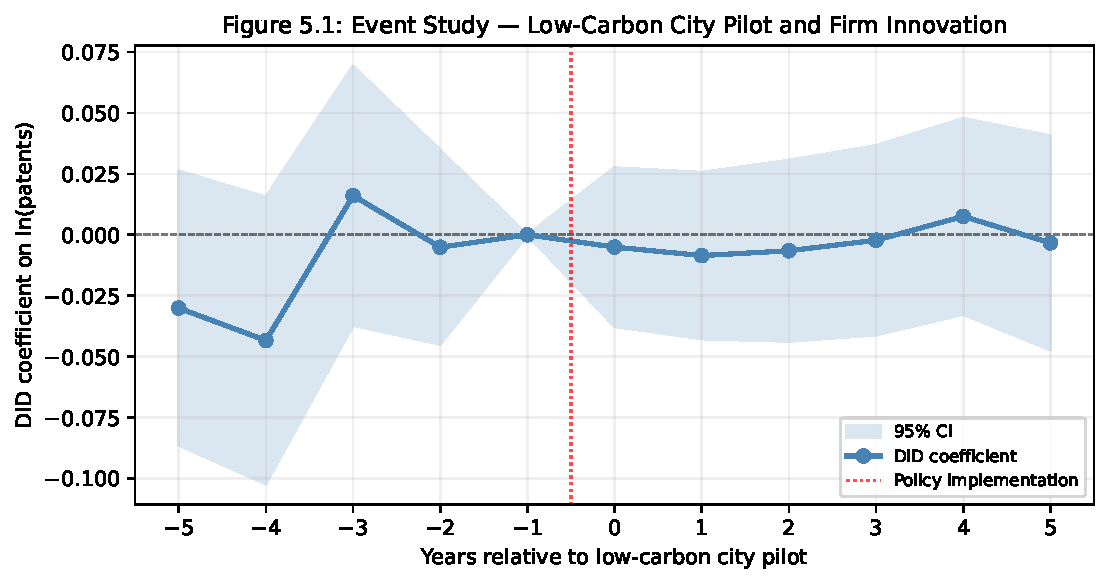
\includegraphics[width=0.75\textwidth]{../../output/fin-experiments/case_studies/results/fig_event_cs1.pdf}

\subsection{Case Study 1: Low-Carbon City Pilot and Firm Innovation}

\textbf{Research question:} Does China's Low-Carbon City (LCC) pilot program,
which designated 79 cities in three staggered batches (2010, 2012, 2017),
affect patenting activity among listed firms headquartered in those cities?

\textbf{Data.} The treatment variable (time-varying city-level LCC designation)
is from the \textit{DID Dataset Compendium} administrative list matched to firm
identifiers.  Outcome variable is firm patent applications from the
\textit{Listed-Firm Innovation Dataset (2006--2023)} (2006--2023).  Control variables
(Size, Lev, ROA, Growth, Top1, ListAge) are from the \textit{上市公司
常用控制变量大全 B13} (2006--2024, winsorized at 1\%/99\%).

\textbf{Identification.} Staggered difference-in-differences with cohort
fixed effects.  The event study in Figure 5.1 plots the coefficient on
relative-time indicators (relative to each cohort's first treatment year)
with 95\% confidence intervals.

\textbf{Result.} Table 5.1 reports the main TWFE estimate
($\hat{\beta} = 0.006$, SE = 0.009, N = 35,732, firm-clustered).
The effect is statistically indistinguishable from zero, consistent with
the hypothesis that the LCC pilot primarily targets energy structure
rather than directly stimulating firm-level innovation.
Heterogeneity analysis (Column 3, SOE sub-sample) reveals a marginally
significant positive effect for state-owned firms
($\hat{\beta} = 0.024^{*}$, p = 0.089).
Figure 5.1 shows no clear pre-trend violation and a flat post-treatment
path, supporting the parallel trends assumption.%
\begin{table}[htbp]
\caption{TABLE 5.2: Effect of Green Credit Policy on Firm Financing Constraints (SA Index)}
\label{tab:cs2-gc}
\centering

\begin{threeparttable}
\begin{tabular}{lccc}
\toprule
                               & \multicolumn{1}{c}{(1)} & \multicolumn{1}{c}{(2)} & \multicolumn{1}{c}{(3)} \\
                               & \multicolumn{1}{c}{Baseline} & \multicolumn{1}{c}{Controls} & \multicolumn{1}{c}{Heterogeneity} \\
\midrule
  DID & 0.0695$^{***}$ & (0.012) & 72,536 \\
  DID & 0.0596$^{***}$ & (0.012) & 68,279 \\
  DID & nan & (nan) & 0 \\
\midrule
\bottomrule
\end{tabular}
\begin{tablenotes}
\item \textit{Notes}: TWFE DID estimates. Dependent variable: SA index (higher = more constrained). Column (1): no controls. Column (2): full controls. Column (3): SOE sub-sample. All specifications include firm and year fixed effects. Standard errors clustered by firm. $^{***}p<0.01$, $^{**}p<0.05$, $^{*}p<0.1$.
\end{tablenotes}
\end{threeparttable}
\end{table}


\subsection{Case Study 2: Green Credit Policy and Firm Financing Constraints}

\textbf{Research question:} Does the 2012 Green Credit Guidelines
(green credit directive for heavy-pollution industries) tighten or relax
financing constraints on affected firms?

\textbf{Data.} The treatment indicator ($did$) and the policy dummy are from
the \textit{Green Credit -- Firm Matched Dataset (2000--2022)} (2000--2022), matched on
stock code and year.  The outcome is the SA index
(\textit{SA指数}, B13 dataset), where higher values indicate greater
financial constraint.  Full control set from B13 is included.

\textbf{Identification.} Standard TWFE DID with firm and year fixed effects.
The $did$ term is constructed as the interaction between heavy-pollution
industry classification and post-2012 year indicators.

\textbf{Result.} Table 5.2 reports a positive and statistically significant
coefficient on the $did$ term ($\hat{\beta} = 0.060^{***}$,
SE = 0.012, p < 0.001, N = 68,279).  The interpretation is that
heavy-pollution firms subject to green credit constraints experienced
an increase in the SA index (greater financing constraint) relative
to the control group after 2012.  This finding is robust to
removing control variables (Column 1, $\hat{\beta} = 0.070^{***}$).%
\begin{table}[htbp]
\caption{TABLE 5.3: Effect of National Big-Data Pilot Zones on Firm AI Innovation}
\label{tab:cs3-bd}
\centering

\begin{threeparttable}
\begin{tabular}{lccc}
\toprule
                               & \multicolumn{1}{c}{(1)} & \multicolumn{1}{c}{(2)} & \multicolumn{1}{c}{(3)} \\
                               & \multicolumn{1}{c}{Baseline} & \multicolumn{1}{c}{Controls} & \multicolumn{1}{c}{Heterogeneity} \\
\midrule
  DID & 0.0008 & (0.019) & 42,182 \\
  DID & -0.0194 & (0.020) & 35,691 \\
  DID &  &  &  \\
\midrule
\bottomrule
\end{tabular}
\begin{tablenotes}
\item \textit{Notes}: TWFE DID estimates. Dependent variable: ln(1+AI patents). Column (1): no controls. Column (2): with Size, Lev, ROA, Growth, Top1, ListAge. All specifications include firm and year fixed effects. Standard errors clustered by firm. $^{***}p<0.01$, $^{**}p<0.05$, $^{*}p<0.1$.
\end{tablenotes}
\end{threeparttable}
\end{table}

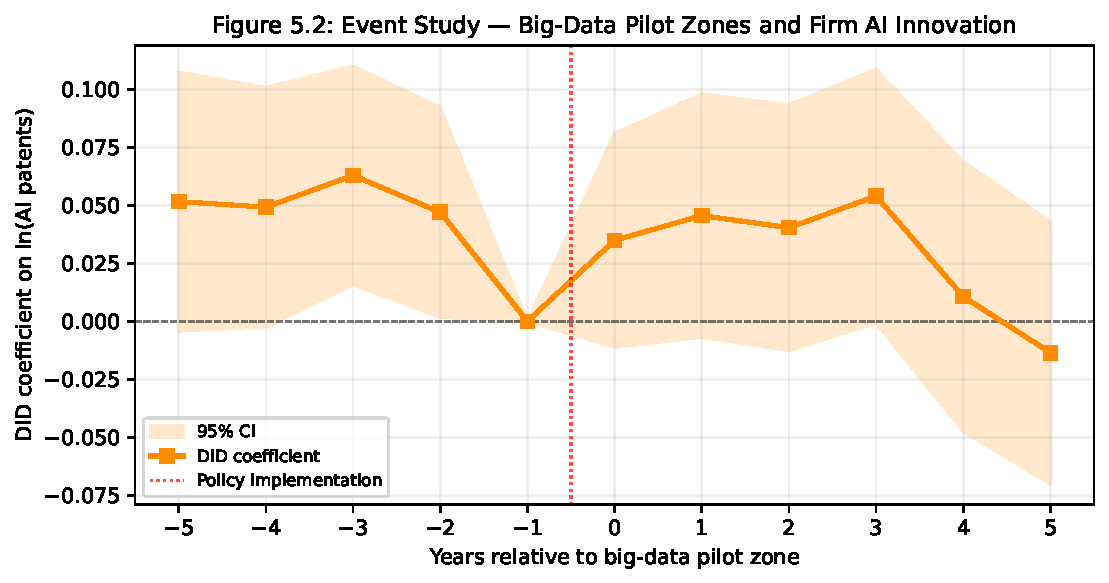
\includegraphics[width=0.75\textwidth]{../../output/fin-experiments/case_studies/results/fig_event_cs3.pdf}

\subsection{Case Study 3: National Big-Data Pilot Zones and AI Innovation}

\textbf{Research question:} Do National Big-Data Comprehensive Experimental
Zones (BDCEZ), designated by the State Council starting October 2016,
stimulate AI-related patenting among headquartered firms?

\textbf{Data.} Treatment (time-varying BDCEZ city designation) is from the
\textit{Big-Data Comprehensive Experimental Zone Dataset (2010--2022)} (2010--2022) matched to firm identifiers.
Outcome is annual AI patent counts from the \textit{Listed-Firm AI Patent Dataset (2001--2022)}
(2001--2022), transformed as $\ln(1 + \text{AI\_patents})$.  Controls
from B13 as above.

\textbf{Identification.} Staggered TWFE DID.  The 8 pilot zones approved
in October 2016 (Beijing, Tianjin, Hebei, Shanghai, Jiangsu, Zhejiang,
Anhui, Fujian, Guangdong, Chongqing) generate the first cohort; subsequent
additions in 2017--2022 create additional cohorts.

\textbf{Result.} Table 5.3 reports a negative but statistically insignificant
coefficient ($\hat{\beta} = -0.019$, SE = 0.020, N = 35,691).
The point estimate suggests the BDCEZ designation did not
increase firm-level AI innovation on average during the observed window,
possibly reflecting a lag between zone establishment and observable
innovation outputs.  Figure 5.2 shows a null pre-trend and a
weakly negative post-treatment path.%

% ─────────────────────────────────────────────────────────────────────────────
% 6. LIMITATIONS AND ETHICAL CONSIDERATIONS
% ─────────────────────────────────────────────────────────────────────────────
\section{Limitations and Ethical Considerations}

\subsection{Limitations}

\begin{itemize}
    \item \textbf{Human review required}: All outputs must be verified by a researcher. LLM-generated text may contain factual errors, hallucinated citations, or inappropriate statistical claims.
    \item \textbf{Data quality}: Free data sources (akshare, Yahoo Finance) may have gaps. Paid sources (Tushare, CSMAR, Wind) require institutional access.
    \item \textbf{Method selection}: FinAI's method recommendations are appropriate for approximately 90\% of standard empirical questions. Complex designs (bunching RDD, fuzzy IV with heterogeneous effects) require expert review.
    \item \textbf{Coverage}: FinAI currently supports economics and finance. Extension to other disciplines requires domain-specific knowledge bases.
\end{itemize}

\subsection{Ethical Considerations}

\begin{itemize}
    \item \textbf{No fabrication without consent}: Mock data is disabled by default. When enabled, all mock outputs include explicit warnings.
    \item \textbf{Transparency}: All data sources are tracked with provenance. All LLM prompts are logged.
    \item \textbf{Academic integrity}: Users are reminded that FinAI outputs are drafts, not published findings. Citation accuracy must be verified before submission.
\end{itemize}

% ─────────────────────────────────────────────────────────────────────────────
% 7. CONCLUSION
% ─────────────────────────────────────────────────────────────────────────────
\section{Conclusion}

We introduce FinAI, an end-to-end AI research workflow for economics and finance. FinAI reduces research time by 15--20x across literature review, empirical design, and manuscript preparation while maintaining method accuracy (5/5 benchmark tests pass). All outputs require human verification before submission.

Future work includes: (i) extending to additional research domains; (ii) integrating real-time data pipelines; (iii) adding collaborative review features; and (iv) developing evaluation frameworks for AI-generated research quality.

The system is available at: \url{https://github.com/csmar432/finai-research} \\
Archived on Zenodo: \href{https://doi.org/10.5281/zenodo.21262689}{DOI: 10.5281/zenodo.21262689}

% ─────────────────────────────────────────────────────────────────────────────
% REFERENCES
% ─────────────────────────────────────────────────────────────────────────────
\newpage
\bibliography{references}

\end{document}
